% K字 例3：矩形 ABCD，AB=6, BC=8，P∈BC，∠APQ=90°，Q∈CD，BP=2，求 CQ=2
\documentclass[tikz,border=4pt]{standalone}
\usepackage{ctex}
\usepackage{amsmath}
\usetikzlibrary{calc}
\begin{document}
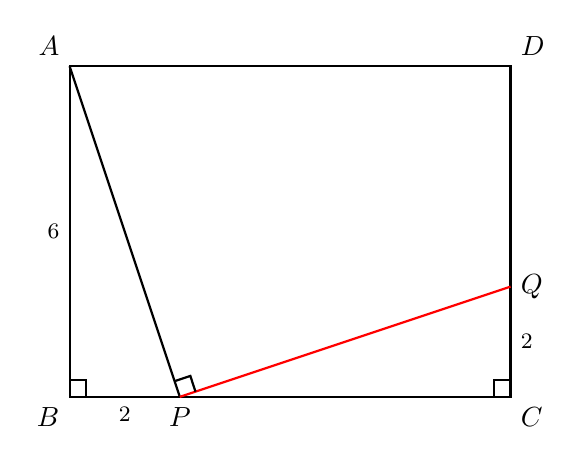
\begin{tikzpicture}[scale=0.7, thick]
  % AB=6, BC=8. A 左上, B 左下, C 右下, D 右上. BC 是直线 l.
  \coordinate (A) at (0,6);
  \coordinate (B) at (0,0);
  \coordinate (C) at (8,0);
  \coordinate (D) at (8,6);
  \coordinate (P) at (2,0);
  \coordinate (Q) at (8,2);
  \draw (A)--(B)--(C)--(D)--cycle;
  \draw (A)--(P);
  \draw[red] (P)--(Q);
  % 三直角
  \draw ($(B)+(0,0.3)$) -- ($(B)+(0.3,0.3)$) -- ($(B)+(0.3,0)$);
  \draw ($(C)+(-0.3,0)$) -- ($(C)+(-0.3,0.3)$) -- ($(C)+(0,0.3)$);
  % ∠APQ 在 P：AP 方向 atan2(6,-2)≈108.4°, PQ 方向 atan2(2,6)≈18.4°
  \draw ($(P)+({0.3*cos(108.4)},{0.3*sin(108.4)})$) --
        ($(P)+({0.3*cos(108.4)+0.3*cos(18.4)},{0.3*sin(108.4)+0.3*sin(18.4)})$) --
        ($(P)+({0.3*cos(18.4)},{0.3*sin(18.4)})$);
  \node[above left] at (A) {$A$};
  \node[below left] at (B) {$B$};
  \node[below right] at (C) {$C$};
  \node[above right] at (D) {$D$};
  \node[below] at (P) {$P$};
  \node[right] at (Q) {$Q$};
  \node[left] at ($(A)!0.5!(B)$) {\footnotesize $6$};
  \node[below] at ($(B)!0.5!(P)$) {\footnotesize $2$};
  \node[right] at ($(C)!0.5!(Q)$) {\footnotesize $2$};
\end{tikzpicture}
\end{document}
